\section{Kaskadowe klasyfikatory cech Haar'a (Maciej Plewka)}

Wybraną metodą zaimplementowaną w celu rozpoznawania obiektów są kaskady Haar'a. Jest to bardzo skuteczny i szybki sposób detekcji oparty na kaskadowych klasyfikatorach cech. Metoda ta działa sprawnie przetwarzając wideo w czasie rzeczywistym, więc w doskonale sprawdza się w naszym przypadk, ze względu na szybki czas działania. Takie rozwiązanie detekcji obiektów został zaprezentowany prez Paula Viola i Michael Jones w jedej z ich prac naukowych \cite{violaJones}

\subsection{Cechy Haar'a}
Proces detekcji obiektów oparty jest o tzw. Cechy Haara. Są to prostokąty takie jak przedstawiono na rysunku \ref{fig:cechyHaara}. Zawierają one informacje na temat różnicy wartości pikseli na zaznaczonych obszarach, dodatkowo wartości te są przeskalowane odwrotnie porcjonalnie do ich wielkości
\begin{figure}[H]
\centering
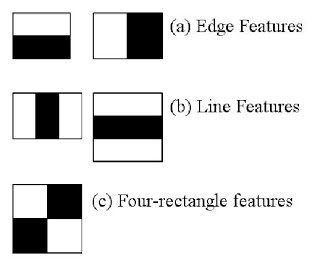
\includegraphics[scale=0.5]{imgs/cechy.jpg}
\caption{{Cechy Haara Źródło:} \cite{faceDetectionOpenCV}}
\label{fig:cechyHaara}
\end{figure}

Zdefiniowane zostały 3 rodzaje cech. Pierwsza \ref{fig:cechyHaara} a jest przedstawiana jako różnica sum pixeli znajdujących się na zaznaczonych prostokątach. Drugi \ref{fig:cechyHaara} b  Opisywany jest jako różnica sumy skrajnych prostokątów i prostokątu wewnętrznego. Trzecia cecha reprezentowana jako cztery prostokąty jest różnicą sum prostokątów leżących na jednej przekątnej. Każda z takich cech może zawierać informacje między innymi na temat krawędzi i różnych zmian w teksturze na podstawie przejść z jasnych do ciemnych fragmentów i odwrotnie. Dla obrazu o rozmiarze 24x24 można wyznaczyć łącznie 162336 cech wszystkich typów przedstawionych na rysunku \ref{fig:cechyHaara}. Jednak do detekcji obiektu potrzebne jest tylko kilkadziesiąt lub kilkaset z nich. Algorytm \ref{alg:sumaPikseli} pokazuje obliczanie wszystkich cech Haar'a typu \ref{fig:cechyHaara} a.

\begin{algorithm}[H]
\caption{Wyznaczanie możliwych cech Haar'a typu \ref{fig:cechyHaara}a}
\label{alg:sumaPikseli}
\begin{algorithmic} 
\DontPrintSemicolon
\STATE $x, y$: \tcp*{wymiary zdjęcia, szerokosc i wysokosc}
\FOR{$i = 1$ \TO $x$ } 
\FOR{$j = 1$ \TO $y$}
\FOR{$w = 1$ \TO $i+h-1$}
\FOR{$h = 1$ \TO $j+2w-1$}
\STATE Oblicz sumę pikseli ${S_{1}}$ w [i, i + h -1] x [j, j + w - 1]
\STATE Oblicz sumę pikseli $S_2$ w [i, i + h -1] x [j+w, j + 2w - 1]
\STATE zapisz cechę o parametrach (i, j, w, h): ${S_{1}}$ - ${S_{2}}$
\ENDFOR
\ENDFOR
\ENDFOR
\ENDFOR
\end{algorithmic}
\end{algorithm}

\subsection{Obliczanie wartości sumy pikseli}

Każdorazowe obliczanie wartości sumy pikseli dla każdego prostokąta wewnątrz zdjęcia byłoby bardzo kosztowne i algorytm detekcji wykonywałby się w długim czasie. W celu skrócenia czasu zastosowano tak zwany Obraz scałkowany (ang. Integral Image).
Pojęcie to polega na obliczeniu w pierwszej kolejności sumy pikseli dla każdego punktu (x,y) zdjęcia w odniesieniu do lewego górnego rogu. Wartości te obliczane są analogicznie do algorytmu Summed-area table używanego w grafice \cite{sumAreaTable}. Wzór \ref{eq1} przedstawia w jaki sposób obliczana jest wartość obrazu scałkowanego dla punktu (x, y)

\begin{equation} \label{eq1}
ii(x,y) = \sum_{x'<x, y'<y}^{} i(x', y')
\end{equation}

Wyznaczanie sumy zdjęcia scałkowanego to dwie rekurencyjne operacje wektorowe, na kolumnach i wierszach.
Posiadając obliczone wartości sumy pikseli dla w każdym punkcie obrazu w którym szukamy obiektu możemy łatwo obliczyć wartość pikseli wewnątrz każdego prostokąta w stałym czasie.

\begin{figure}[H]
\centering
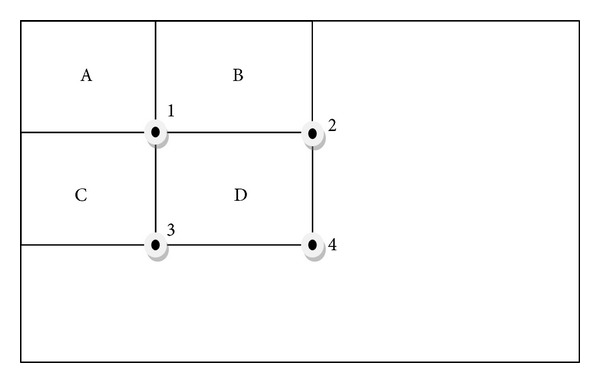
\includegraphics[scale=1.4]{imgs/sumPixels.png}
\caption{Obliczanie sumy wartości pikseli Źródło: \cite{sumPixelsDoc}}
\label{fig:obrazScalkowany}
\end{figure}

Rysunek \ref{fig:obrazScalkowany} przedstawia schemat obrazu, po transformacji do obrazu scałkowanego dla którego próbujemy wyznaczyć sumę pikseli w wewnętrznym prostokącie. W celu obliczenia sumy pikseli dla zaznaczonego prostokąta D musimy uwzględnić wartości sum 4 prostokątów. Suma pikseli dla prostokąta A jest równa wartości zdjęcia scałkowanego w punkcie 1,
Analogicznie w punkcie 2 opisuje wartość sumy dla prostokąta A + B, w punkcie 3 dla prostokąta A + C, natomiast w punkcie 4 dla prostokąta A + B + C + D. Do wyznaczenia sumy pikseli w prostokącie D potrzebujemy zatem wartości zdjęcia scałkowanego w punktach opisującym ten prostokąt. I tak dla przedstawionego schematu suma pikseli w prostokącie D jest równa 4 - 2 -3 + 1.
Wyznaczenie tej wartości dla każdego prostokąta zatem zawsze jest wykonane w stałym czasie, są to zawsze te same operacje dodawania i odejmowania.

\subsection{Proces uczenia mocnych klasyfikatorów}

Każdy klasyfikator włączony do kaskady jest złożony z wielu tzw. Słabych klasyfikatorów. Każdy z nich jest pojedynczą cechą Haar’a która została włączona do klasyfikatora w procesie uczenia. Pojedynczy klasyfikator zwykle nie jest w stanie jednoznacznie sklasyfikować obiektu. W celu usprawnienia skuteczności detekcji za pomocą cech stosuje się tak zwany Boosting. Celem tego zabiegu jest stworzenie klasyfikatora, którego ocena będzie składała się z ocen wielu klasyfikatorów odpowiednio przeskalowane w stosunku do ich skuteczności określonym w etapie uczenia. 

\begin{figure}[H]
\centering
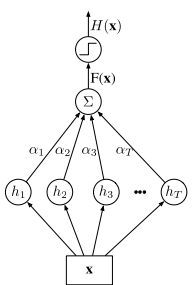
\includegraphics[scale=0.6]{imgs/mocny.png}
\caption{Działanie mocnego klasyfikatora Źródło: \cite{AdaBoostClasifire}}
\label{fig:klasyfikatorMocny}
\end{figure}

Rysunek \ref{fig:klasyfikatorMocny} przedstawia działanie mocnego klasyfikatora. Na wejściu podane jest zdjęcie X które jest analizowane przez każdą cechę $h$. Następnie wynik każdej cechy(możliwe \{1, -1\}) jest rozmnażany przez jej współczynnik, potem wyniki są sumowane. Jeśli suma jest większa od 0 uznane zostanie, że jest to obiekt jeśli wartość jest mniejsza X nie jest szukanym obiektem.

Mocne Klasyfikatory otrzymywane są w procesie uczenia maszynowego, do którego potrzebny będzie zbiór danych uczących. W skład takiej bazy będą wchodziły zdjęcia, na których znajduje się szukany obiekt, tak zwane zdjęcia pozytywne, oraz zdjęcia na których nie ma obiektu, tak zwane zdjęcia negatywne. Dodatkowo dane muszą posiadać etykiety które informują czy na zdjęciu znajduje się obiekt czy też nie. W tym przypadku kaskady Haar’a są otrzymywane poprzez implementacje algorytmu AdaBoost jest to jeden ze sposobów uczenia z nadzorem. To iteracyjny algorytm, w każdej iteracji wybierany  jest jeden słaby klasyfikator w tym przypadku cecha Haar’a, która najskuteczniej klasyfikuje obiekt. Dene, które zostały źle sklasyfikowany przez wybraną cechę zostają obciążone większymi wagami, by w następnych iteracjach kolejne klasyfikatory musiały radzić sobie szczególnie dobrze ze zdjęciami błędnie oznaczonymi przez poprzednio wybrane cechy. Tak dobrane słabe klasyfikatory łącznie tworzą silny klasyfikator, który jest włączany do kaskady. Na wejście algorytmu podany jest zestaw danych uczących wraz z etykietami \{$x_{i}$, $y_{i}$\} $x_{i}$ jest kolejnym zdjęciem a $y_{i}$ jest etykietą \{1, -1\}. Zbiór danych liczy n elementów.

\begin{algorithm}[H]
\caption{AdaBoost}
\begin{algorithmic} 
\DontPrintSemicolon
\STATE $D_k(i)$: \tcp*{przykładowa waga elementu $i$ klasyfikatora $k$}
\STATE $\alpha_k$:\tcp*{ waga klasyfikatora $k$}
\STATE $\forall_i$: $D_1(i) \gets$ ${1} \over {n}$ \tcp*{pocztkowe wagi danych}
\FOR{$k = 1$ \TO $K$ } 
\STATE $\forall h$ $\epsilon_k \gets$ $\sum_{i:y\neq h(x_i)}^{} $ $D_k(i)$ \tcp* {obliczanie błędu dla każdego klasyfikatora}
\STATE $h_k \gets argmin(\epsilon_k(h))$ \tcp* {wybór klasyfiatora z najmniejszym błędem}
\IF{$\epsilon_k \geq$ $1 \over 2$} 
\STATE stop \tcp*{jeśli klasyfikator ma 50\% błędu stop}
\ELSE
\STATE $\alpha_k \gets $ $1 \over 2$ $1- \epsilon_k \over \epsilon_k$
\STATE $D_{k+1}(i) \gets$ $D_k(i)e^{-y_i\alpha_k h_k(x_i)} \over Z_k$
\ENDIF
\ENDFOR
\STATE $H_{final}(x) = sgn(\sum_{k=1}^{K} \alpha_k h_k(x))$
\end{algorithmic}
\end{algorithm}

Ocena skuteczności klasyfikatora opiera się na tak zwanej macierzy pomyłek (z ang. Confusion Matrix), która definiuje współczynniki określające:
\begin{itemize}
    \item Ilość dobrych klasyfikacji jako obiekt
    \item Ilość złych klasyfikacji jako obiekt
    \item Ilość dobrych klasyfikacji jako nie obiekt
    \item Ilość złych klasyfikacji jako nie obiekt
\end{itemize}

Na podstawie tych danych obliczany jest współczynnik dobrze sklasyfikowanych obiektów w stosunku do liczby zdjęć pozytywnych, dalej określany jako TPR ( z ang. true positive rate). Obliczany jest także współczynnik błędnych decyzji jako stosunek liczby błędnie sklasyfikowanych jako obiekt do liczby zdjęć negatywnych, dalej określany jako FPR(z ang. false positive rate)

\subsection{Kaskada klasyfikatorów mocnych}
W celu dodatkowego poprawienia skuteczności zaproponowano zastosowanie kaskady klasyfikatorów, która jest czymś na wzór drzewa decyzyjnego. Każdy z mocnych klasyfikatorów otrzymanych na podstawie działania algorytmy AdaBoost jest jednym z elementów kaskady. Aktualnie poszukiwany obszar jest sprawdzany przez kolejne klasyfikatory. Na wejście kaskady podawany jest analizowany obszar. Pierwszy klasyfikator analizuje fragment wszystkimi cechami które wchodzą w jego skład. Jeśli klasyfikator stwierdzi że we wskazanym obszarze znajduje się obiekt fragment zostaje poddany analizie przez następny klasyfikator w kaskadzie. Jeśli fragment zostanie niesklasyfikowany przez któryś element kaskady zostaje podjęta jednoznaczna decyzja dla całej kaskady o braku obiektu. O obecności szukanego wzorca w kaskadzie, muszą wskazać wszystkie elementy kaskady. Podczas uczenia kolejne etapy wybierają do klasyfikatora mocnego cechy z coraz mniejszej puli jest ich zatem coraz więcej w kolejnych elementach kaskady. 
	
Sama detekcja jest oparta na sprawdzaniu kolejnych fragmentów zdjęcia przesuwając miejsce badanego fragmentu po całym obrazie. Analiza fragmentów, które są tłem obiektu trwa stosunkowo krótko ponieważ o braku obiektu powinny stwierdzić pierwsze elementy kaskady, które składają się z mniejszej ilości cech niż końcowe etapy. Analiza przy użyciu końcowych etapów kaskady jest wykorzystana prawie tylko w sytuacjach obiektu podobnego do szukanego, okolicy szukanego obiektu bądź znalezienia wzorca.
Kosztowna analiza za pomocą wszystkich cech wchodzących w skład kaskady jest wykonywana tylko dla mniejszej części zdjęcia, co sprawia, że algorytm jest szybki.
